\documentclass[11pt,a4paper]{article}

\usepackage[utf8]{inputenc}
\usepackage[T1]{fontenc}
\usepackage[english]{babel}
\usepackage{amsmath,amssymb}
\usepackage{graphicx}
\usepackage{xcolor}
\usepackage{booktabs}
\usepackage{caption}
\usepackage{subcaption}
\usepackage[margin=2.4cm]{geometry}
\usepackage{hyperref}
\hypersetup{colorlinks=true,linkcolor=blue!50!black,urlcolor=blue!50!black}
\graphicspath{{figures/}}

\title{%
\textbf{Development of an Automatic Design Optimization Platform\\
for a 2D Heat-Conduction System Using FreeFEM++}\\[4pt]
\large HEAT-COND benchmark --- FreeFEM++ and Python}
\author{Laurent Zhu \and Alexandre Le Droucpeet}
\date{Optimization and Numerical Analysis (MATH6304P-260-M01) --- Spring 2026\\
Shanghai Jiao Tong University --- SPEIT}

\begin{document}
\maketitle

\begin{abstract}
\noindent We develop a compact, automatic design-optimization platform for the 2D
steady-state HEAT-COND heat-conduction benchmark, coupling a FreeFEM++ $P_1$ finite-element
solver with a Python optimization driver. Through seven systematic studies we show that the
objective is smooth and unimodal with a \emph{boundary} optimum at
$\mathbf{x}^\star=(1,1,1,1,1,0.01)$, giving $J^\star\approx0.730$ at mesh density~50 ---
roughly an $850\%$ improvement over the uniform design. Of the three compared methods
(Nelder--Mead, Differential Evolution, and an Adam\,$\rightarrow$\,L-BFGS hybrid),
\textbf{Nelder--Mead is the most efficient and is chosen as the platform default}; Differential
Evolution serves as a global-optimality check, and the gradient hybrid illustrates the value
of adaptive preconditioning on this ill-conditioned problem. We further extend the benchmark with
a material-cost objective whose Pareto front shows that $32\%$ of the conductive material can be
saved for under $1\%$ performance loss.
\end{abstract}

\section{Introduction and Project Objective}
This project develops a compact, automatic design-optimization platform for a two-dimensional
steady-state heat-conduction problem, the HEAT-COND benchmark drawn from the reduced-basis
literature~\cite{ballout2024}. The platform integrates, within a single reproducible workflow,
the five required components: a finite-element solver written in FreeFEM++, an objective-evaluation
module, a Python optimization driver, a graphical user interface, and a numerical-analysis
framework for comparing optimization strategies.

The scientific goal is to couple the solution of an elliptic partial differential equation (PDE)
posed on a non-trivial 2D geometry with an automated parametric optimization loop, and to
determine, through systematic experiments, \emph{which optimization strategy is best suited to
this problem and why}. As we show, the objective functional is smooth and unimodal with its
optimum located on the boundary of the admissible set; this single structural fact explains the
entire ranking of the methods we tested, and motivates the optimizer chosen as the platform
default.

\section{Mathematical Model}
\subsection{Geometry}
The computational domain $\Omega\subset[0,1]^2$ is a comb-shaped region consisting of a central
vertical \emph{spine} of width $w_s=0.10$ and five pairs of horizontal \emph{fins} of thickness
$t_f=0.06$, centred at $y\in\{0.16,0.32,0.48,0.64,0.80\}$. The inner spine edges are at
$x_g=(1-w_s)/2=0.45$ and $x_d=x_g+w_s=0.55$. Two boundary regions are distinguished:
$\Gamma_{\text{Base}}$, the bottom edge of the spine $\{(x,0):x\in[x_g,x_d]\}$, and
$\Gamma_{\text{Fin}}$, the remainder of $\partial\Omega$ (the spine top, the outer fin tips, and
all fin flanks). The domain, its boundary labels and the $P_1$ mesh are shown in
Fig.~\ref{fig:geom}.

\begin{figure}[h]
\centering
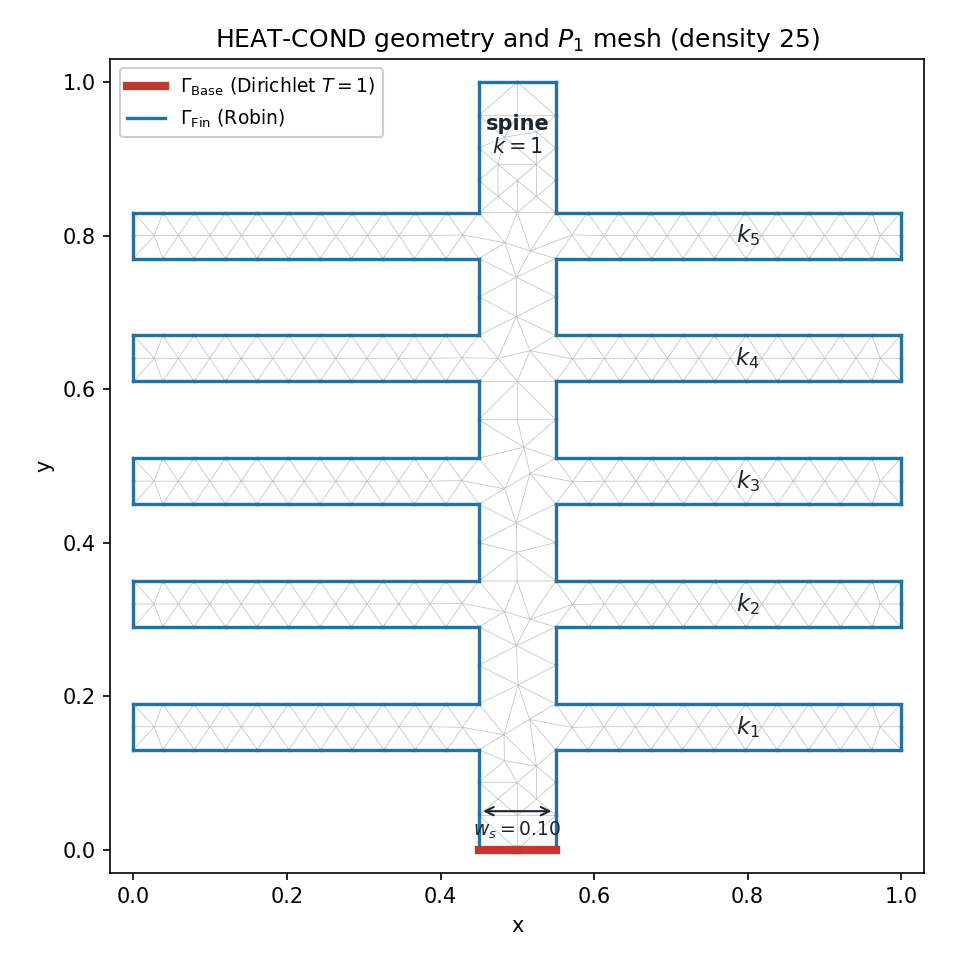
\includegraphics[width=0.6\textwidth]{geometry_mesh.png}
\caption{HEAT-COND geometry and $P_1$ mesh (density 25). The red base $\Gamma_{\text{Base}}$
carries the Dirichlet condition $T=1$; the blue boundary $\Gamma_{\text{Fin}}$ carries the Robin
condition. The central spine has conductivity $k=1$; each fin $i$ has conductivity $k_i$.}
\label{fig:geom}
\end{figure}

\subsection{Governing Equation}
The dimensionless temperature $T$ satisfies the steady-state heat-conduction equation with mixed
(Dirichlet--Robin) boundary conditions:
\begin{equation}
\begin{cases}
-\nabla\cdot\big(k(\mathbf{x})\,\nabla T\big)=0 & \text{in }\Omega,\\[2pt]
T=1 & \text{on }\Gamma_{\text{Base}},\\[2pt]
k(\mathbf{x})\,\dfrac{\partial T}{\partial n}+\mathrm{Bi}\,T=0 & \text{on }\Gamma_{\text{Fin}}.
\end{cases}
\end{equation}
The conductivity $k(\mathbf{x})$ is piecewise constant: $k=1$ in the spine, and $k=k_i$
($i=1,\dots,5$) in fin $i$, counted bottom to top. The Biot number $\mathrm{Bi}$ controls the
convective coupling on $\Gamma_{\text{Fin}}$.

\subsection{Objective and Optimization Problem}
The objective is to maximize the average temperature on the fin boundary,
\begin{equation}
J(\mathbf{x})=\frac{1}{|\Gamma_{\text{Fin}}|}\int_{\Gamma_{\text{Fin}}}T\,\mathrm{d}\Gamma,
\end{equation}
over $\mathbf{x}=(k_1,\dots,k_5,\mathrm{Bi})\in\mathbb{R}^6$ with $k_i\in[0.1,1.0]$ and
$\mathrm{Bi}\in[0.01,1.0]$: $\max_{\mathbf{x}}J(\mathbf{x})$ subject to box constraints. Physically,
a high $J$ means the spine transfers the heat injected at the base ($T=1$) efficiently to the
peripheral fin surfaces.

\section{Numerical Formulation and FreeFEM++ Implementation}
\subsection{Mesh Generation}
The mesh is constructed explicitly with FreeFEM's \texttt{buildmesh} rather than by truncating a
background grid, so that element edges align exactly with the geometry. The boundary is described
as a closed, counter-clockwise polyline of 44 segments / 45 points, traversed by a single indexed
\texttt{border}; the number of subdivisions of each segment is proportional to its Euclidean length
times a global density \texttt{meshsize}. Two boundary labels are assigned: \textbf{label~1} for the
base segment (Dirichlet) and \textbf{label~2} for the rest of the boundary (Robin). Each mesh is
cached as \texttt{cache/mesh\_<size>.msh}. At density 50 the mesh contains 1151 vertices and
1760 triangles (419 vertices at density 25).

\subsection{PDE Solver}
\texttt{solver.edp} reads its parameters through \texttt{getARGV}. The weak form is assembled in the
$P_1$ space $V_h$: find $T\in V_h$ with $T=1$ on $\Gamma_{\text{Base}}$ such that, for all test
functions $v$,
\begin{equation}
a(T,v)=\int_\Omega k\,\nabla T\cdot\nabla v\,\mathrm{d}\Omega
+\int_{\Gamma_{\text{Fin}}}\mathrm{Bi}\,T\,v\,\mathrm{d}\Gamma=0.
\end{equation}
The Dirichlet condition is imposed strongly via \texttt{on(1, T = 1)}; the Robin condition enters
naturally as the boundary integral over label~2. The objective
$J=\int_{\Gamma_2}T\,\mathrm{d}\Gamma/\int_{\Gamma_2}1\,\mathrm{d}\Gamma$ is computed inside the
solver and printed to stdout as \texttt{Objective\_J=<value>}, removing intermediate text files.

\subsection{Python Coupling and Verification}
The Python layer drives FreeFEM through \texttt{subprocess}: \texttt{ensure\_mesh} caches meshes and
\texttt{run\_solver} parses the objective from stdout. To verify the implementation, the $P_1$ weak
form was re-implemented in pure NumPy and compared against FreeFEM on identical cached meshes: at
density 50 the two solvers agree to six significant digits at the optimal corner ---
$J(1,1,1,1,1,0.01)=0.730396$ in both --- and the vertex/triangle counts match exactly. This
cross-check validates the operator and the objective, and lets the optimizer comparison below be
reproduced without FreeFEM.

\section{Optimization Strategy}
The driver wraps every algorithm behind a uniform interface returning a normalized dictionary
(\texttt{best\_J}, \texttt{best\_x}, \texttt{n\_eval}, \texttt{time}, full \texttt{history}); random
methods use a fixed seed. After a preliminary screening we retained \textbf{three complementary
methods}, one per family:
\begin{itemize}
  \item \textbf{Nelder--Mead (NM)} --- local, deterministic simplex in dimension 6; gradient-free,
  sensitive to the start, very cheap.
  \item \textbf{Differential Evolution (DE)} --- global, population-based, gradient-free; robust but
  the most expensive.
  \item \textbf{Adam $\rightarrow$ L-BFGS-B} --- a two-phase gradient hybrid: Adam (finite-difference
  gradient, per-coordinate adaptive step) drives the iterate into a good region, then L-BFGS-B
  refines with native bound handling.
\end{itemize}
Because the objective is a black-box PDE solve, the gradient phase uses central finite differences,
costing $2\times6=12$ extra evaluations per gradient in 6D. The experimental design is implemented
in the notebook \texttt{comparison\_methods.ipynb} as seven self-contained studies; the DE
hyperparameter study averages each configuration over three independent seeds.

\section{Numerical Results}
The reference initial design is $\mathbf{x}_0=(0.5,\dots,0.5)$, for which $J_0\approx0.077$.
Unless stated otherwise, comparisons use mesh density~25; the ranking is identical at density~50.

\subsection{Comparison of the Three Methods and the Optimal Design (Study 1)}
\begin{table}[h]
\centering
\caption{Comparison of the three methods from the common start $\mathbf{x}_0=0.5$ (density 25).}
\begin{tabular}{lrrrl}
\toprule
Method & $J^\star$ & $n_{\text{eval}}$ & Time (s) & Design $\mathbf{x}^\star$\\
\midrule
\textbf{Nelder--Mead} & \textbf{0.73417} & \textbf{115} & 0.28 & $(1,1,1,1,1,0.01)$\\
Adam $\rightarrow$ L-BFGS & 0.73417 & 373 & 0.90 & $(1,1,1,1,1,0.01)$\\
Differential Evolution & 0.73411 & 768 & 1.86 & $(1,0.996,0.986,1,1,0.01)$\\
\bottomrule
\end{tabular}
\end{table}

All three methods reach the same global optimum
$\mathbf{x}^\star=(1,1,1,1,1,0.01)$ --- all conductivities at their upper bound and the Biot
number at its lower bound, a vertex of the admissible box. At density 50 this corner gives
$J^\star=0.730396$, an $\approx850\%$ improvement over $J_0$. Nelder--Mead reaches it at the lowest
cost; Differential Evolution is the most expensive and stops just short of the exact corner
(Fig.~\ref{fig:e1}). The effect of the optimization on the temperature field is shown in
Fig.~\ref{fig:tfields}: the initially cold fins ($T$ down to $0.003$ at the tips) become uniformly
hot ($T\ge0.633$).

\begin{figure}[h]
\centering
\begin{subfigure}{0.56\textwidth}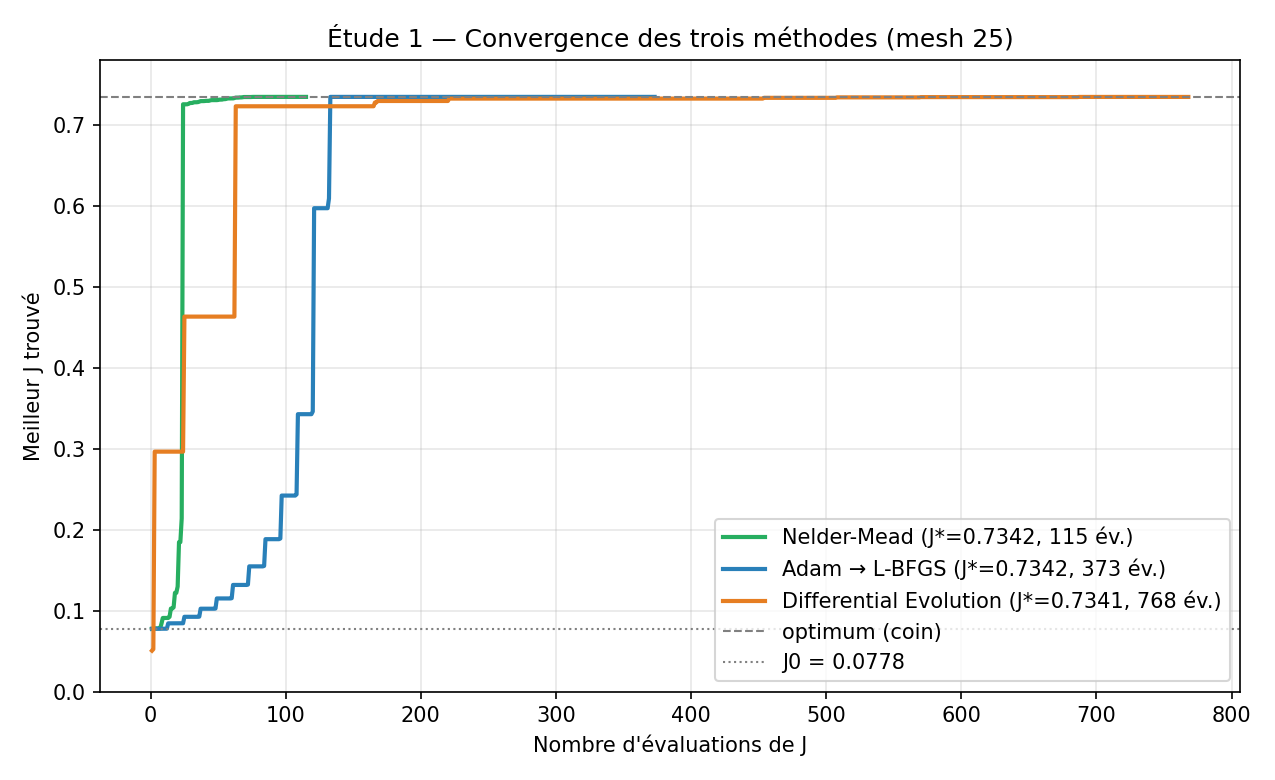
\includegraphics[width=\linewidth]{etude1_convergence.png}\end{subfigure}
\hfill
\begin{subfigure}{0.42\textwidth}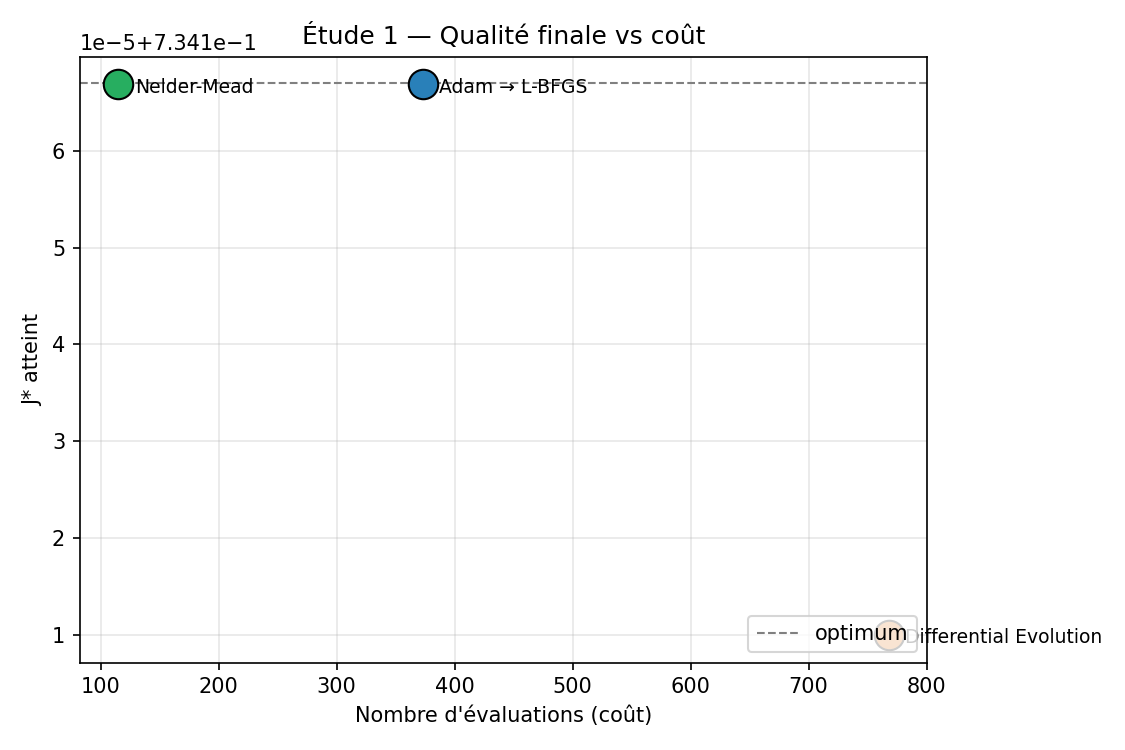
\includegraphics[width=\linewidth]{etude1_pareto.png}\end{subfigure}
\caption{Study 1 --- convergence (left) and quality-vs-cost trade-off (right). All three methods
reach the optimal corner; Nelder--Mead does so in the fewest evaluations.}
\label{fig:e1}
\end{figure}

\begin{figure}[h]
\centering
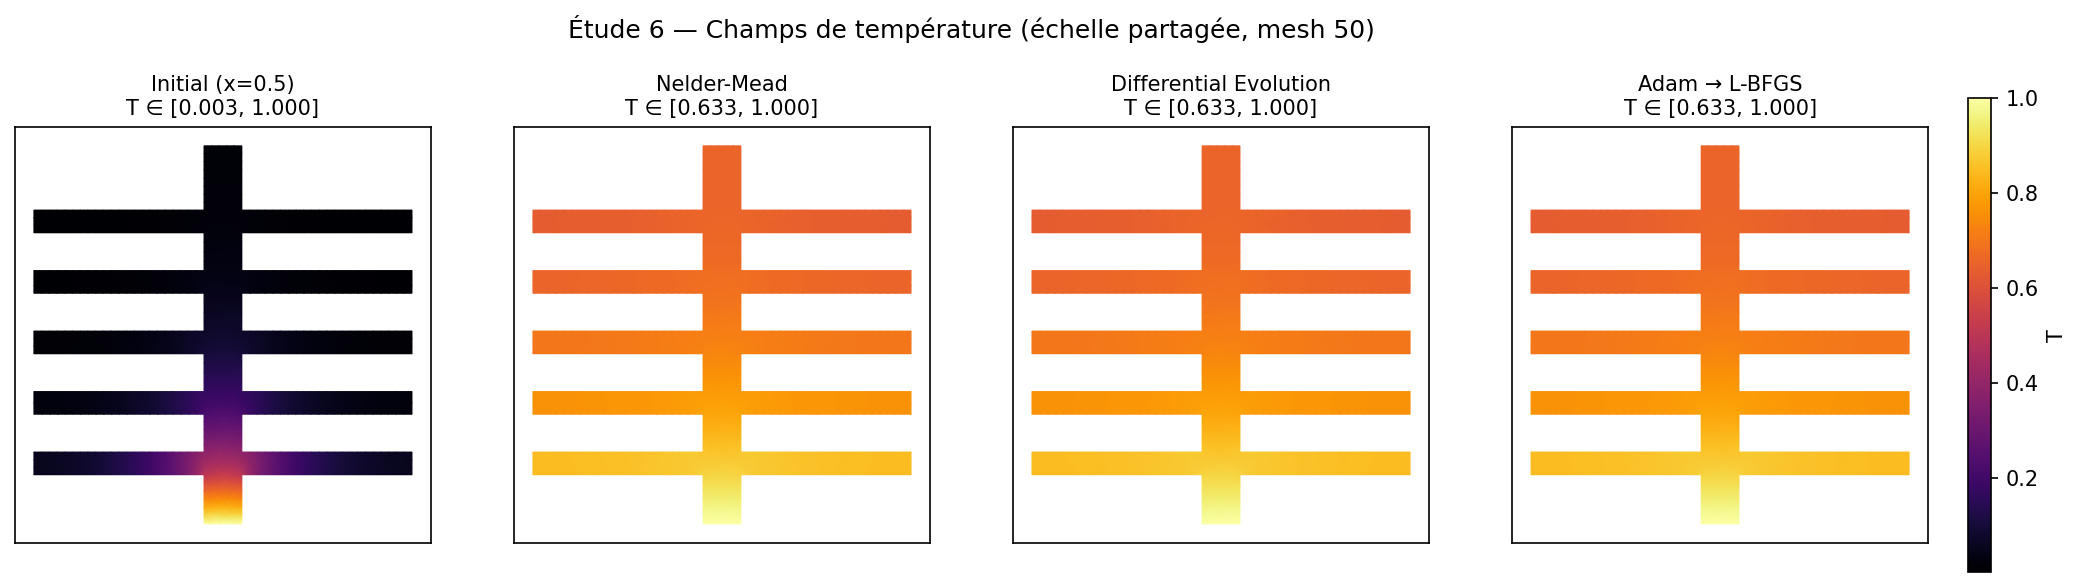
\includegraphics[width=\textwidth]{etude6_T_fields.png}
\caption{Temperature fields (shared colour scale, mesh 50) for the initial design and the three
optimized designs. Optimization raises the minimum fin temperature from $0.003$ to $0.633$.}
\label{fig:tfields}
\end{figure}

\subsection{Mesh-Sensitivity (Study 2)}
\begin{table}[h]
\centering
\caption{Optimized objective (Nelder--Mead) vs mesh density.}
\begin{tabular}{lcccc}
\toprule
Mesh density & 15 & 25 & 40 & 60\\
\midrule
$J^\star$ & 0.7414 & 0.7342 & 0.7313 & 0.7295\\
\bottomrule
\end{tabular}
\end{table}
$J^\star$ decreases monotonically and stabilizes near $0.73$ as the mesh is refined, indicating
approximate mesh-independence by density 50--60; coarse meshes slightly over-estimate the
objective. The wall-clock time grows steeply with density (more degrees of freedom), as shown in
Fig.~\ref{fig:e2}.

\begin{figure}[h]
\centering
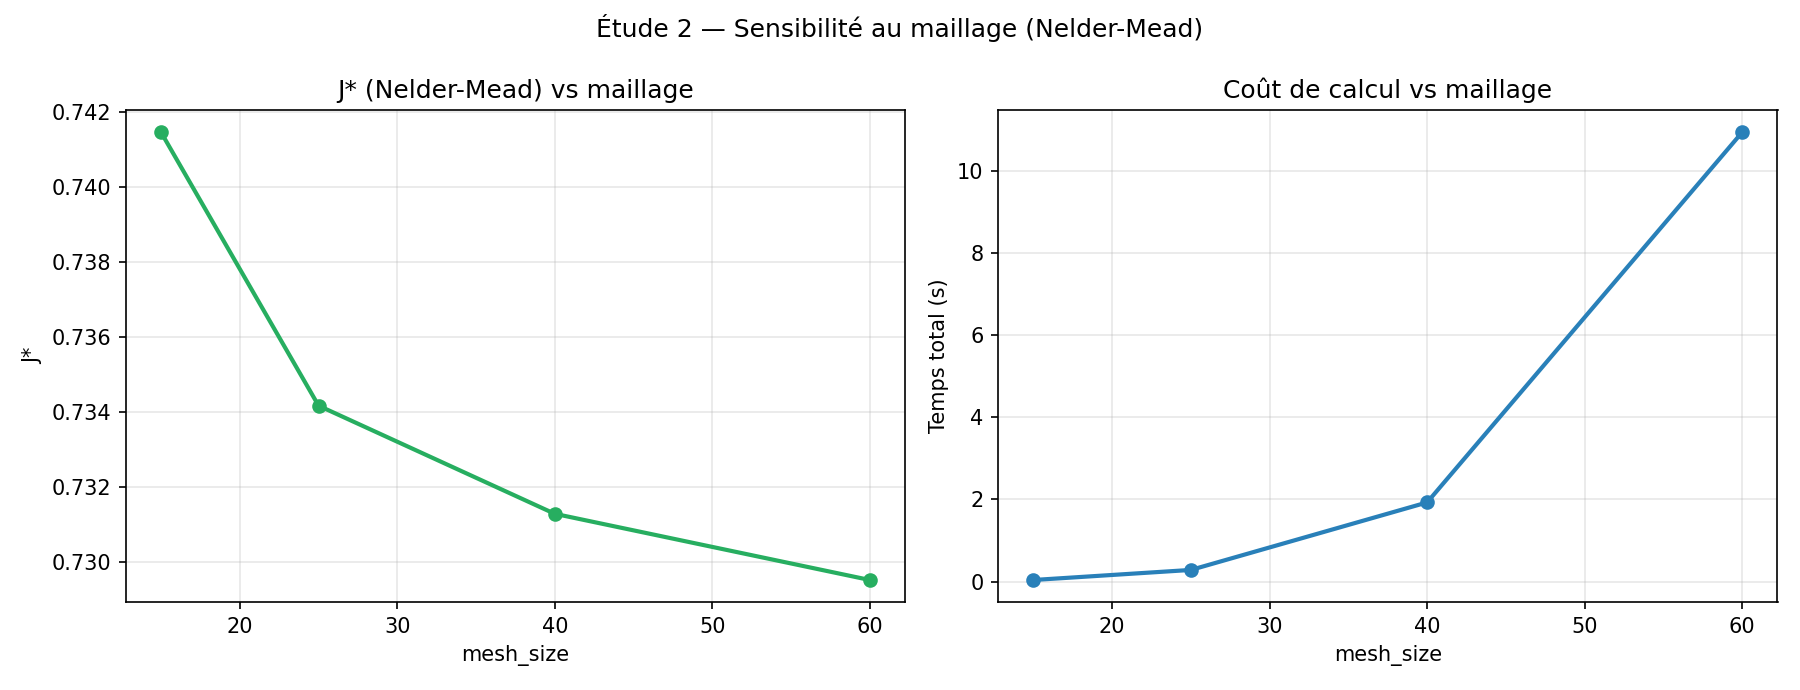
\includegraphics[width=0.9\textwidth]{etude2_mesh.png}
\caption{Study 2 --- mesh-sensitivity of $J^\star$ (left) and computational cost (right).}
\label{fig:e2}
\end{figure}

\subsection{Robustness (Studies 3 and 4)}
Study 3 varies the starting point for the local/gradient methods (NM, Adam); Study 4 varies the
random seed for the only stochastic method (DE). Nelder--Mead is the most reproducible across
starting points (standard deviation $\sim\!10^{-4}$, mean $0.7341$), confirming that the functional
is effectively unimodal. Adam$\rightarrow$L-BFGS reaches the corner from every tested start
(std $\sim\!6\times10^{-4}$), and DE shows a small seed-to-seed spread (std $\sim\!2\times10^{-3}$).
All three are robust; Nelder--Mead is the most stable (Fig.~\ref{fig:e34}).

\begin{figure}[h]
\centering
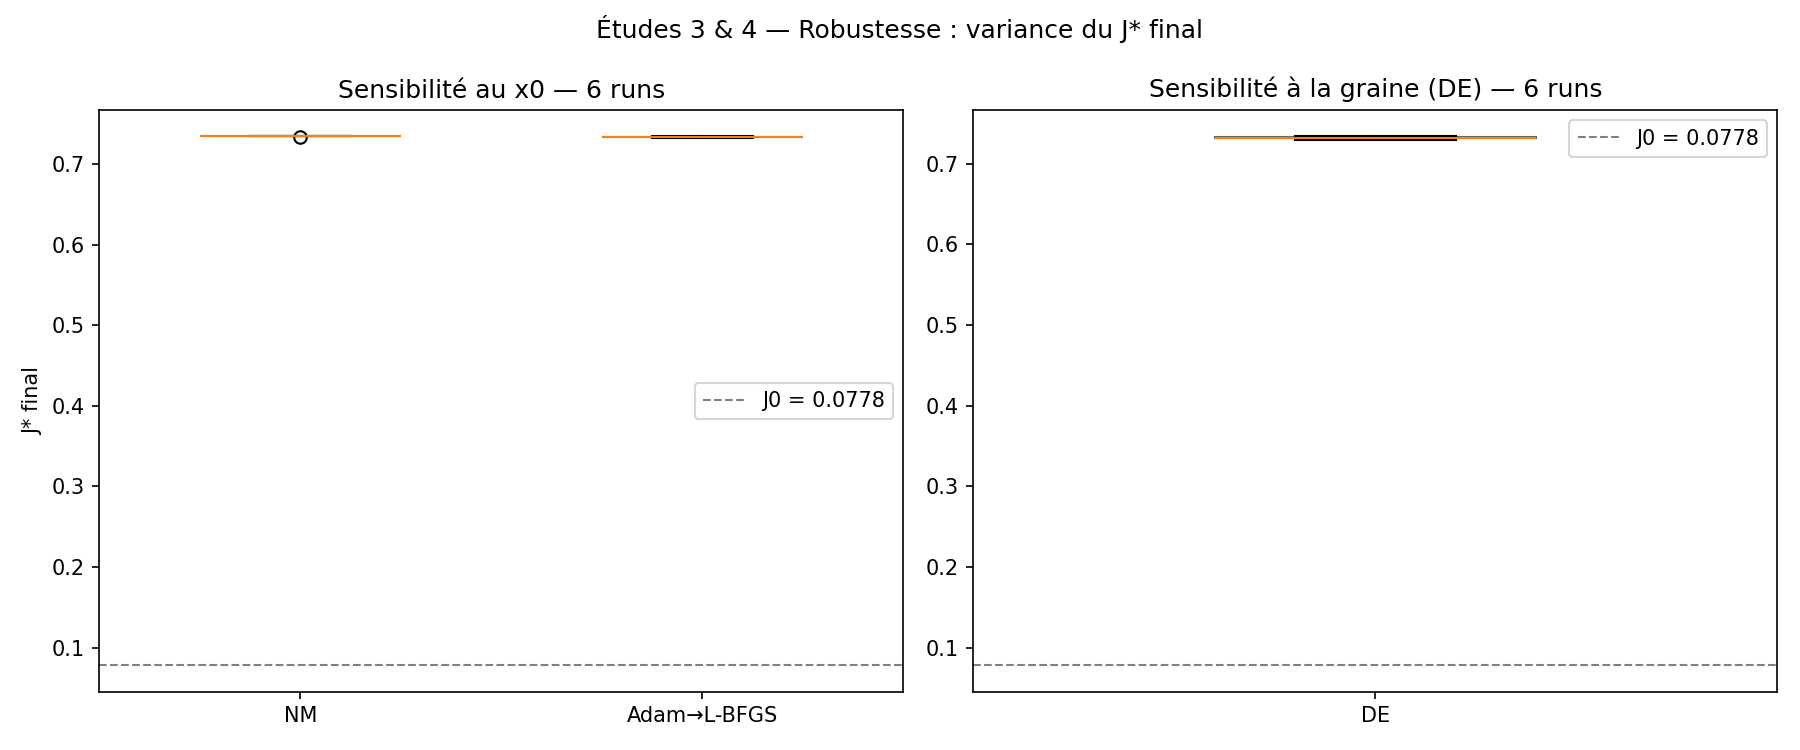
\includegraphics[width=0.85\textwidth]{etude34_robustness.png}
\caption{Studies 3--4 --- variability of $J^\star$ across starting points (NM, Adam) and across
seeds (DE).}
\label{fig:e34}
\end{figure}

\subsection{Differential-Evolution Hyperparameters (Study 5)}
Averaged over three seeds: a larger \texttt{popsize} improves both the mean objective and its
stability (from $0.672\pm0.063$ at \texttt{popsize}$=2$ to $0.717\pm0.002$ at $15$); a low mutation
factor is clearly preferable ($0.718$ at $F=0.3$ vs $0.611$ at $F=1.8$); and \texttt{best1bin} is
the best strategy ($0.701$). These trends are consistent with an exploitation-dominated, unimodal
landscape (Fig.~\ref{fig:e5}).

\begin{figure}[h]
\centering
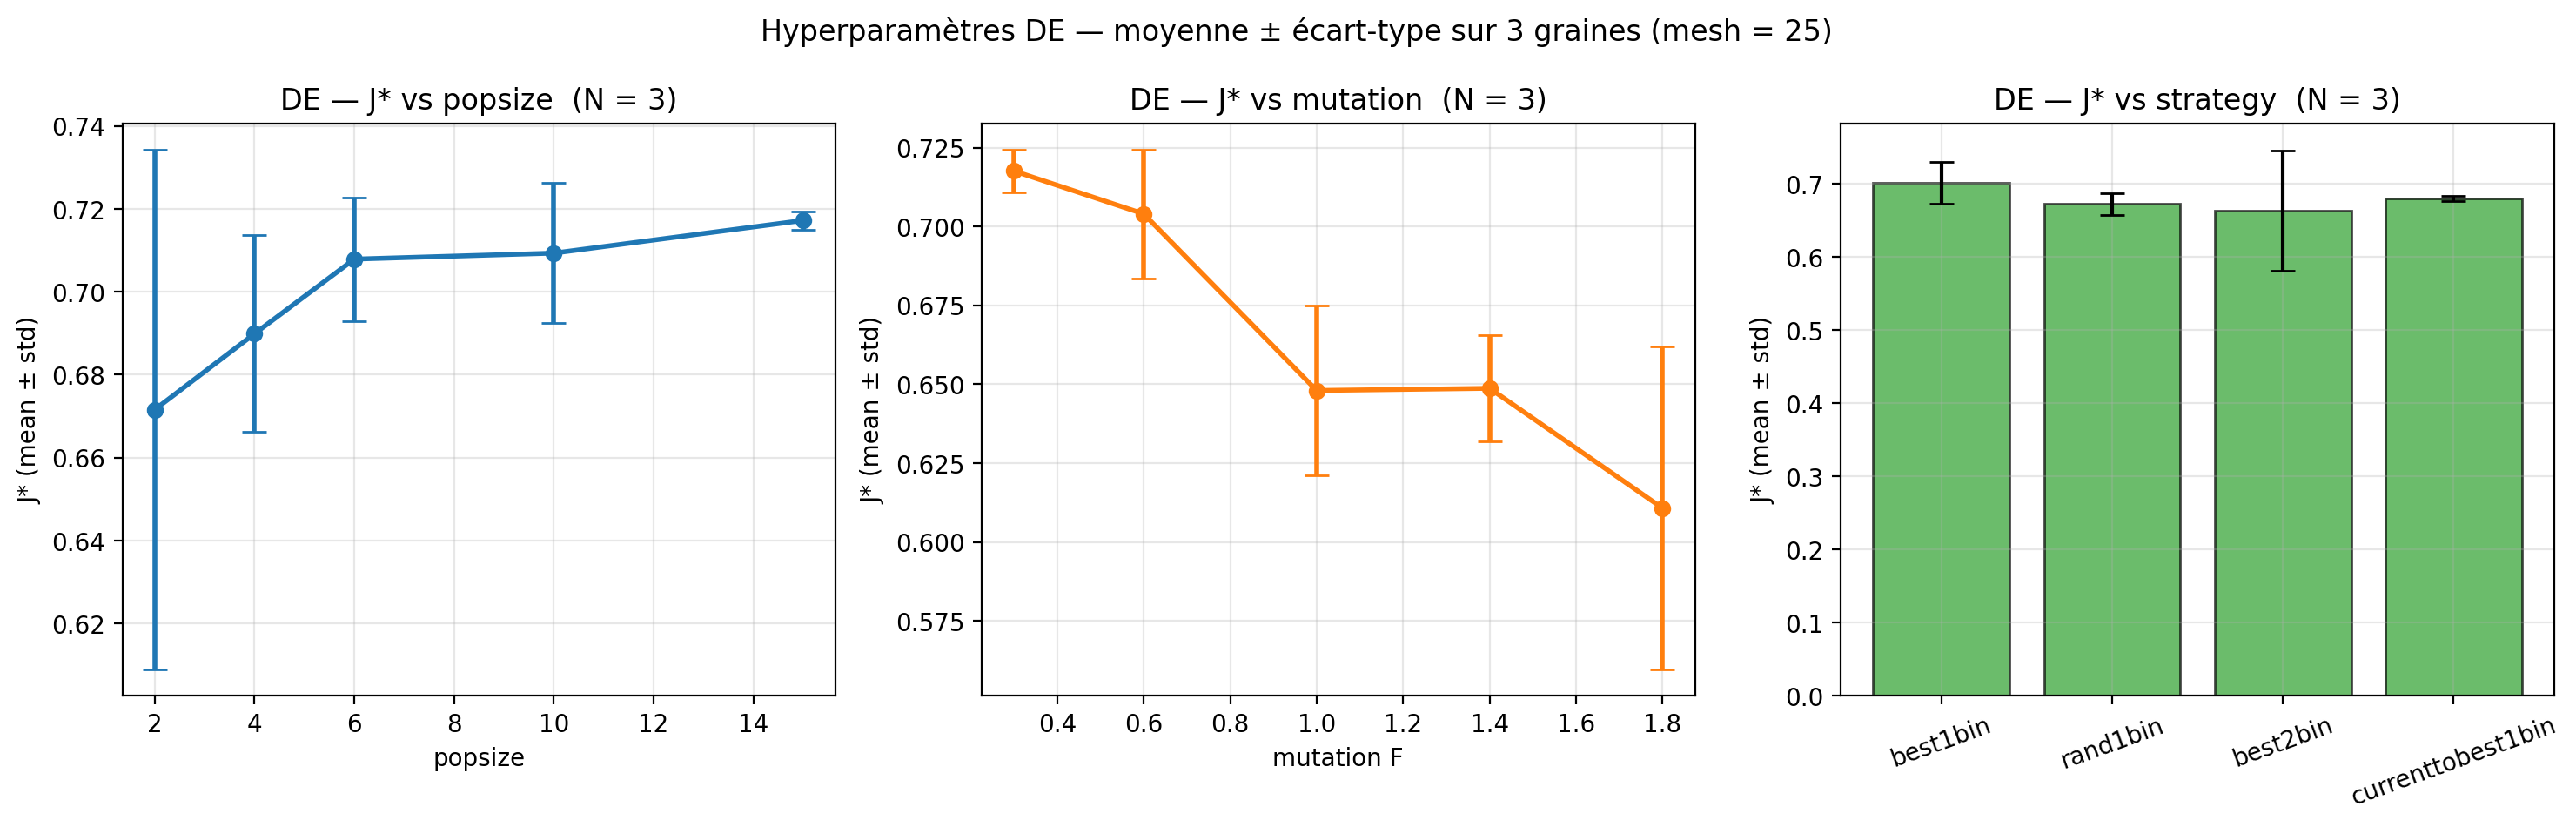
\includegraphics[width=\textwidth]{etude5_DE_hyperparams.png}
\caption{Study 5 --- DE hyperparameters (mean $\pm$ std over three seeds): \texttt{popsize},
\texttt{mutation}, and \texttt{strategy}.}
\label{fig:e5}
\end{figure}

\subsection{The Adam $\rightarrow$ L-BFGS Hybrid and Preconditioning (Study 7)}
This study isolates the contribution of each phase by adding two diagnostic runs from
$\mathbf{x}_0=0.5$:
\begin{table}[h]
\centering
\caption{Diagnostic runs of the gradient hybrid (density 25).}
\begin{tabular}{lrrl}
\toprule
Variant & $J^\star$ & $n_{\text{eval}}$ & Reaches the corner\\
\midrule
Adam $\rightarrow$ L-BFGS & 0.734167 & 373 & yes\\
\emph{Adam alone} & 0.734167 & 360 & yes\\
\emph{L-BFGS-B alone} & 0.721633 & 106 & \textbf{no --- stalls}\\
\bottomrule
\end{tabular}
\end{table}

\textbf{L-BFGS-B alone stalls} at $J=0.722$ with the conductivities stuck near $0.5$, whereas the
hybrid reaches the corner (Fig.~\ref{fig:e7}). A direct probe of the gradient at the stall point
explains why: there $|\partial J/\partial\mathrm{Bi}|\approx19.4$ but
$|\partial J/\partial k_i|\approx0.009$, a ratio of about $2000{:}1$. Once $\mathrm{Bi}$ saturates
at its lower bound, the objective is almost flat in the conductivity directions, and the pure
quasi-Newton method declares convergence. Adam, which normalizes each coordinate by the running
root-mean-square of its gradient, turns this tiny but consistent signal into full-sized steps and
drives the conductivities to $1.0$. This is a textbook illustration of adaptive preconditioning on
an ill-conditioned problem, and it is exactly why the first phase of the hybrid is necessary. The
three methods converge to the same physical design (Fig.~\ref{fig:designs}).

\begin{figure}[h]
\centering
\begin{subfigure}{0.56\textwidth}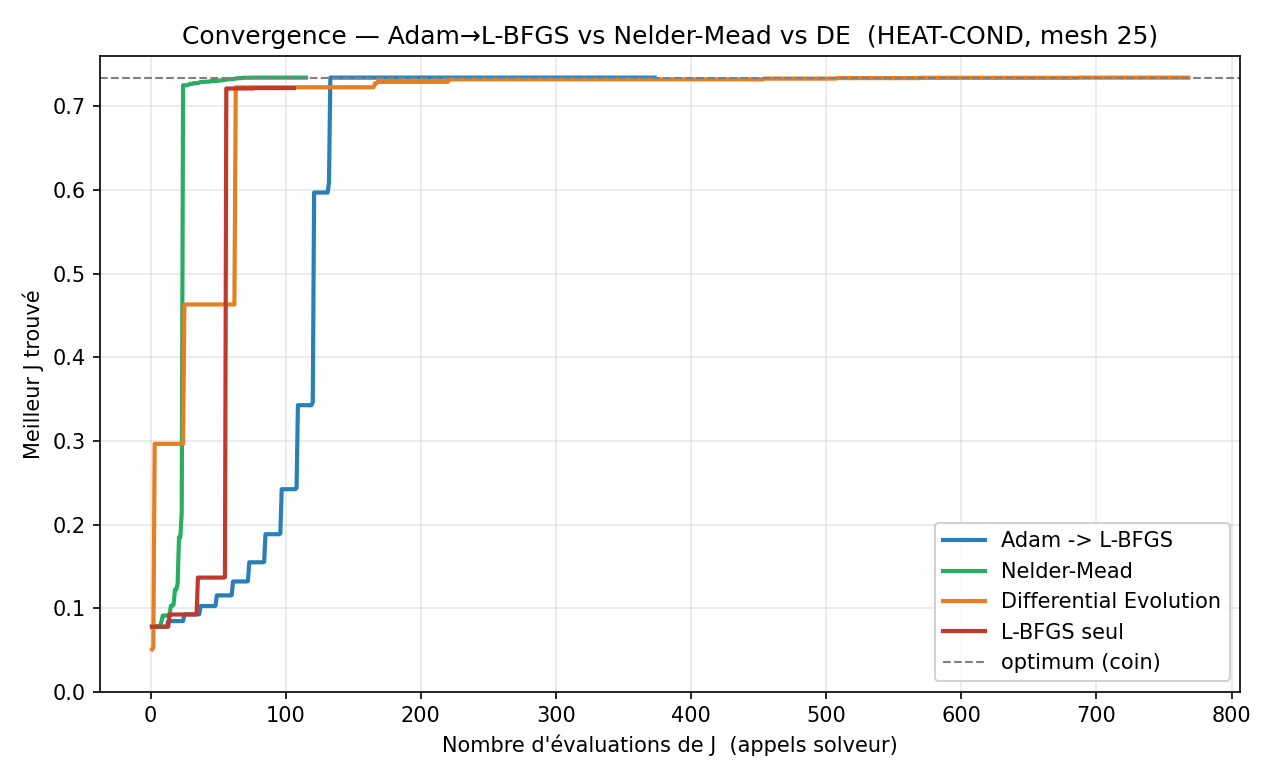
\includegraphics[width=\linewidth]{etude7_convergence.png}\caption{}\label{fig:e7}\end{subfigure}
\hfill
\begin{subfigure}{0.42\textwidth}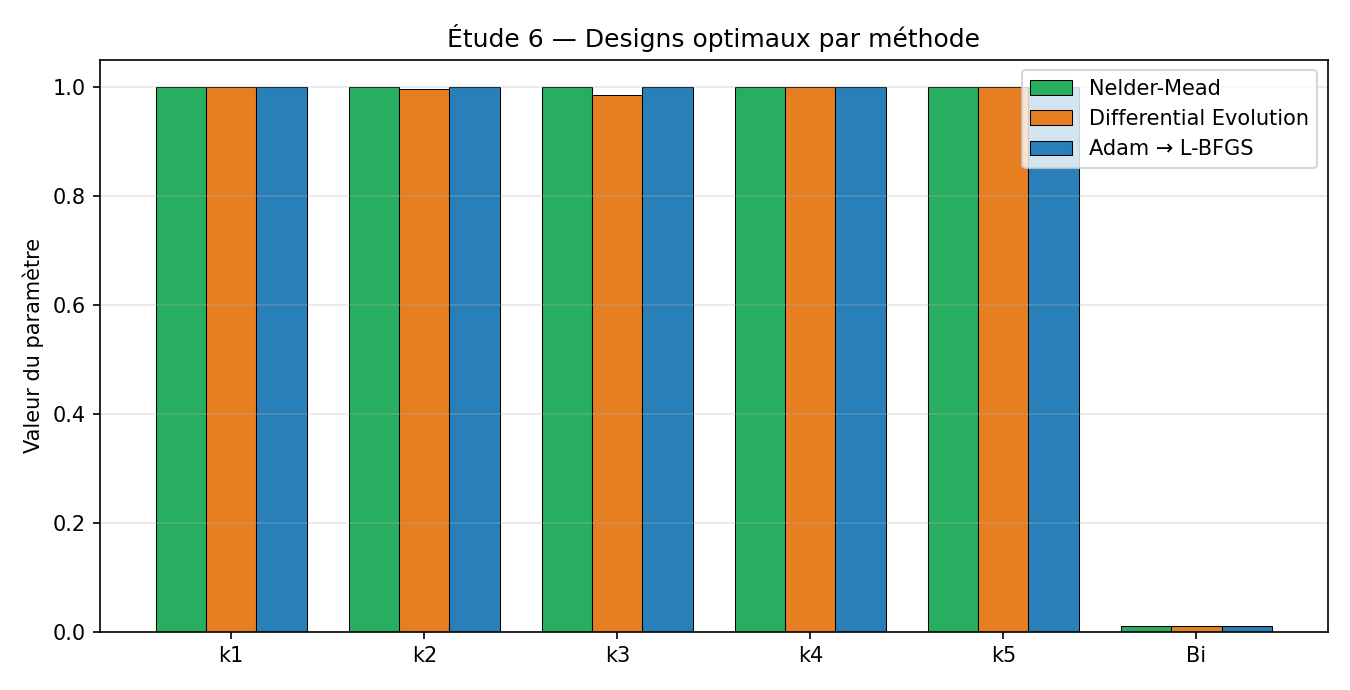
\includegraphics[width=\linewidth]{etude6_designs_bar.png}\caption{}\label{fig:designs}\end{subfigure}
\caption{(a) Study 7 --- convergence of the hybrid against NM and DE; L-BFGS alone (dashed) stalls
below the optimum. (b) Optimal designs found by the three methods: all converge to $k_i\to1$,
$\mathrm{Bi}\to0.01$.}
\end{figure}

\subsection{Extension: Material-Cost Trade-off}
The optimum above is a vertex of the box because higher conductivity is free. A more realistic
design problem penalizes material: we maximize the scalarized objective
$F_\lambda(\mathbf{x})=J(\mathbf{x})-\lambda\bar{k}$, where $\bar{k}=\frac15\sum_i k_i$ is the mean
conductivity (a proxy for material cost), and sweep $\lambda\ge0$ to trace the performance--cost
Pareto front (Fig.~\ref{fig:pareto}). The penalty is evaluated in Python around the solver, so it
ports unchanged to FreeFEM and is exposed in the graphical interface through a single $\lambda$
field.

Two findings stand out. First, the front is strongly concave near the optimum: one can remove
$32\%$ of the conductive material for only a $0.8\%$ loss of performance (the marked knee,
$\bar{k}=0.68$, $J=0.728$ versus $J_{\max}=0.734$). Second, the optimal design becomes non-uniform
with a clear physical ordering $k_1>k_2>k_3>k_4>k_5$ (Fig.~\ref{fig:designlambda}): the fins nearest
the hot base retain their conductivity as $\lambda$ grows, while the upper fins are economized
first; the Biot number stays at its lower bound throughout (it carries no material cost). This
trade-off turns the otherwise trivial corner problem into a genuine multi-objective design study.

\begin{figure}[h]
\centering
\begin{subfigure}{0.52\textwidth}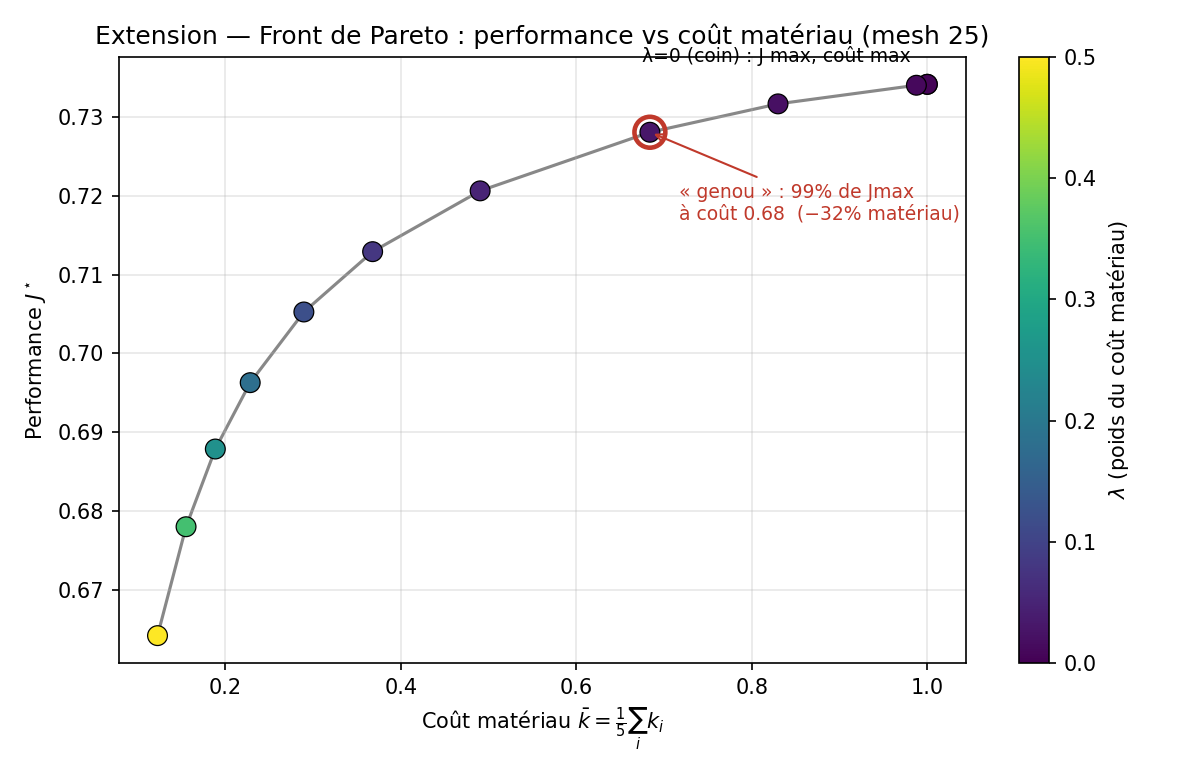
\includegraphics[width=\linewidth]{ext_material_pareto_front.png}\caption{}\label{fig:pareto}\end{subfigure}
\hfill
\begin{subfigure}{0.46\textwidth}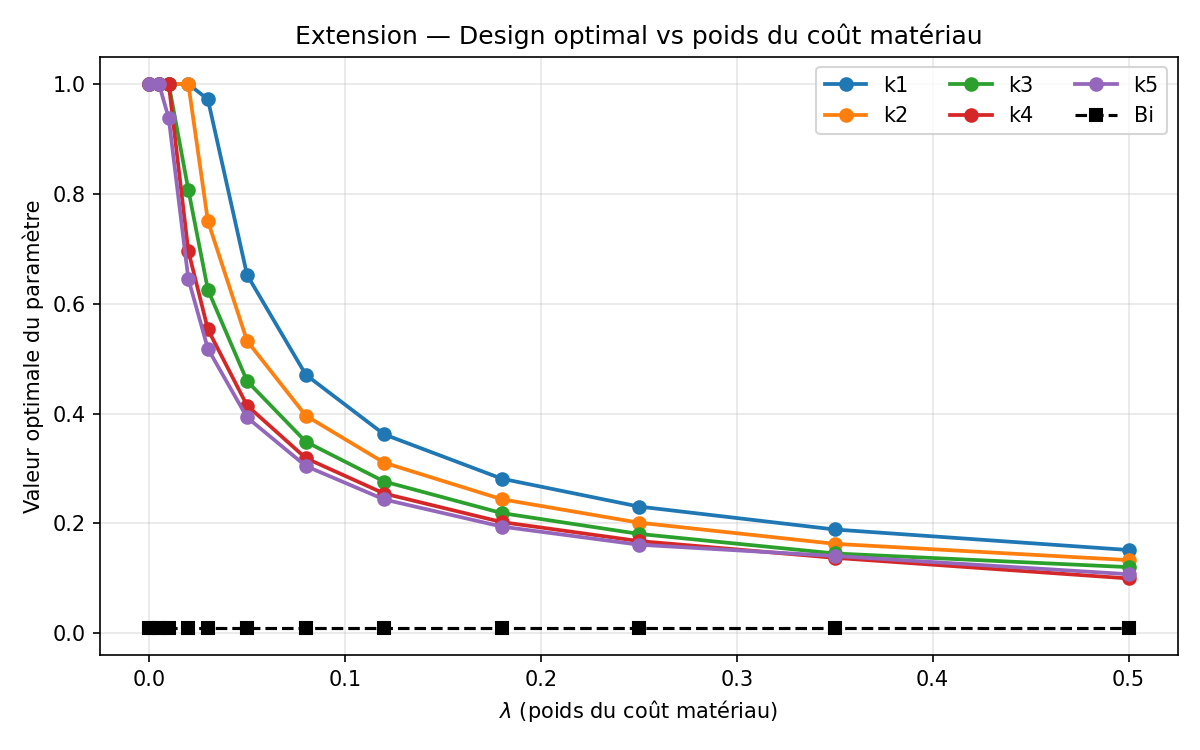
\includegraphics[width=\linewidth]{ext_material_design_vs_lambda.png}\caption{}\label{fig:designlambda}\end{subfigure}
\caption{Material-cost extension. (a)~Performance--cost Pareto front; the marked knee retains
$99\%$ of $J_{\max}$ at $-32\%$ material. (b)~Optimal conductivities versus the cost weight
$\lambda$: the bottom fins ($k_1$) stay conductive longest, the Biot number stays at $0.01$.}
\end{figure}

\subsection{Optimizer Comparison on the Penalized Problem}
Section~5.6 traced the front with a single optimizer. We now repeat the $\lambda$ sweep with all
three methods to check whether the non-trivial (interior) optimum changes the ranking established on
the pure-performance problem. Figure~\ref{fig:methpareto} overlays the three Pareto fronts:
Nelder--Mead and Adam$\rightarrow$L-BFGS coincide, while Differential Evolution lies marginally
inside the front in the mid-cost region, reflecting its fixed, budget-limited search. At a
representative weight $\lambda=0.05$ (near the knee), Nelder--Mead and Adam reach the same scalarized
optimum $F^\star=0.696$, with Nelder--Mead the cheapest ($178$ versus $304$ evaluations), while DE
attains a slightly lower $F^\star=0.695$ at $324$ evaluations (Table~\ref{tab:meth},
Fig.~\ref{fig:methconv}). The conclusion of the pure-performance study therefore carries over to the
constrained problem: all three methods agree on the trade-off, and Nelder--Mead remains the most
efficient default.

\begin{table}[h]
\centering
\caption{Three optimizers on the penalized problem at $\lambda=0.05$ (mesh 25).}
\label{tab:meth}
\begin{tabular}{lrrrr}
\toprule
Method & $J$ & cost $\bar k$ & $F=J-\lambda\bar k$ & $n_{\text{eval}}$\\
\midrule
\textbf{Nelder--Mead} & 0.7206 & 0.490 & \textbf{0.6961} & \textbf{178}\\
Adam $\rightarrow$ L-BFGS & 0.7212 & 0.502 & 0.6961 & 304\\
Differential Evolution & 0.7237 & 0.581 & 0.6947 & 324\\
\bottomrule
\end{tabular}
\end{table}

\begin{figure}[h]
\centering
\begin{subfigure}{0.49\textwidth}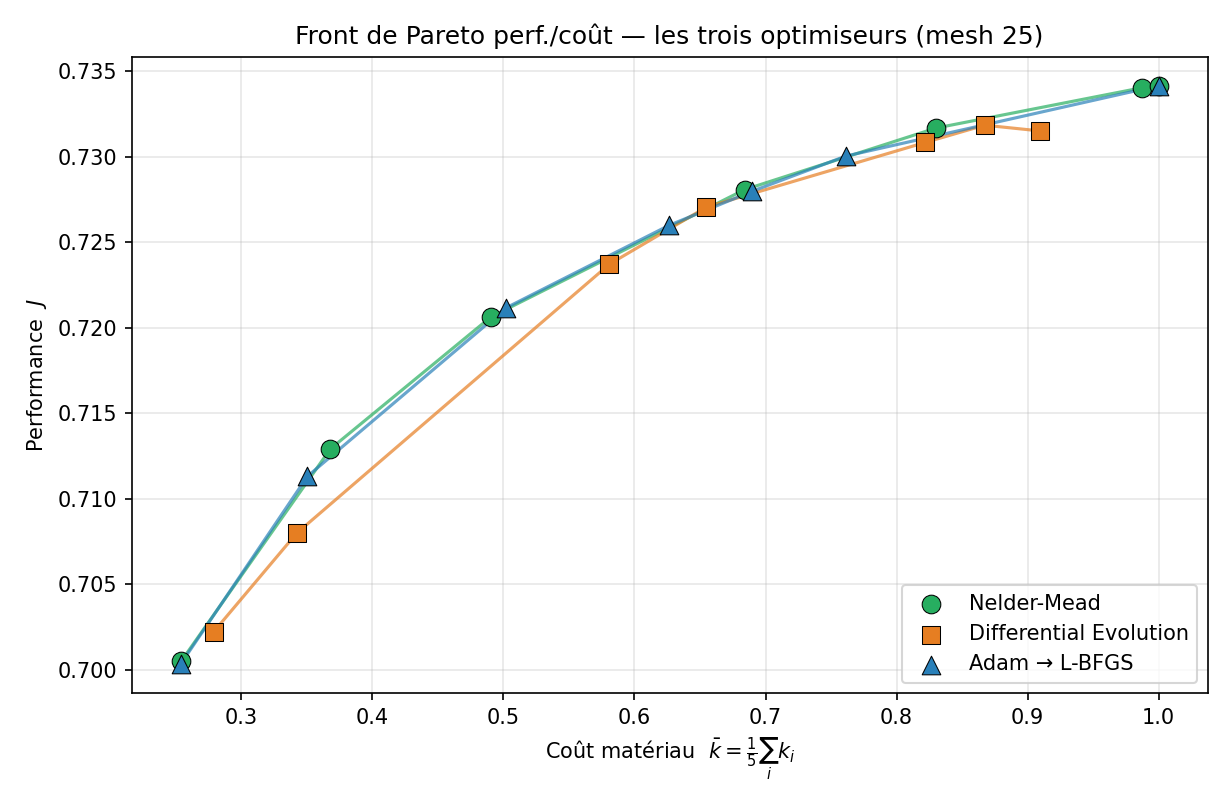
\includegraphics[width=\linewidth]{ext_methods_pareto.png}\caption{}\label{fig:methpareto}\end{subfigure}
\hfill
\begin{subfigure}{0.49\textwidth}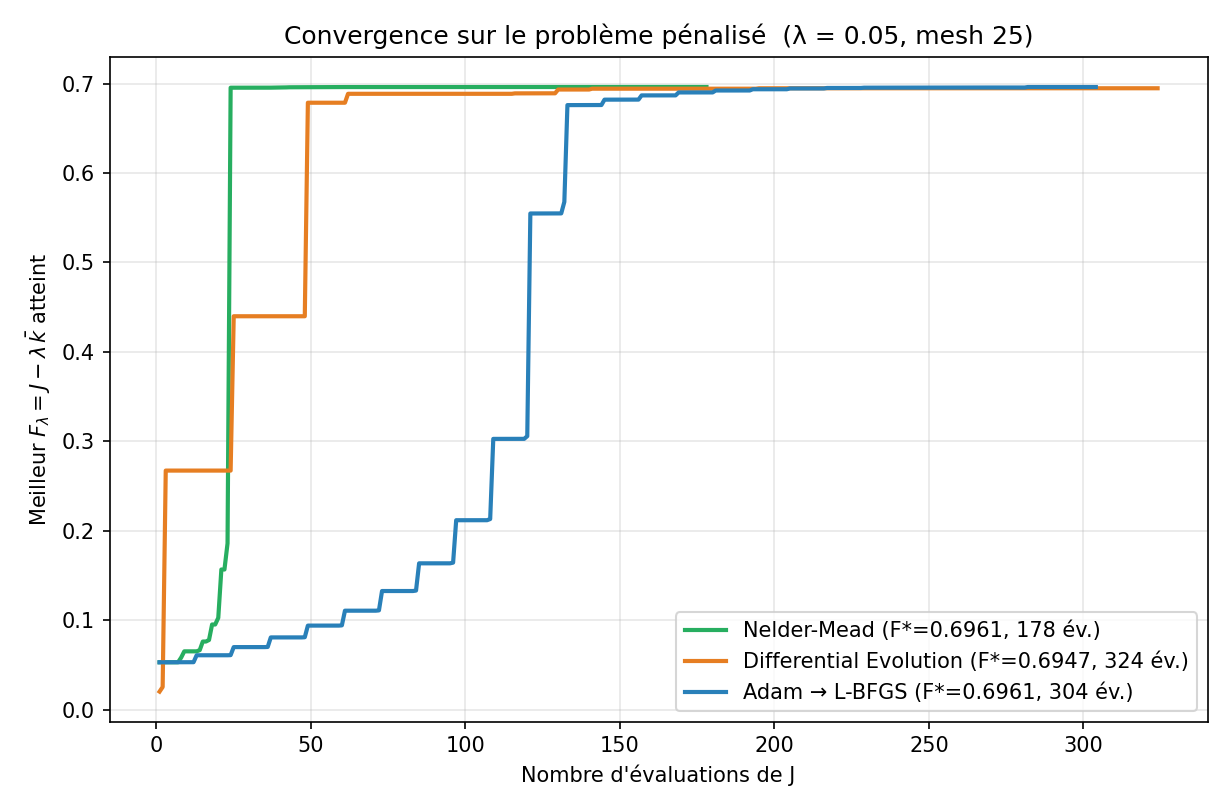
\includegraphics[width=\linewidth]{ext_methods_convergence.png}\caption{}\label{fig:methconv}\end{subfigure}
\caption{The three optimizers on the material-cost problem. (a)~Pareto fronts: Nelder--Mead and
Adam$\rightarrow$L-BFGS coincide; DE lies slightly inside. (b)~Convergence of the scalarized
objective $F_\lambda$ at $\lambda=0.05$: all reach $F^\star\approx0.696$, Nelder--Mead fastest.}
\end{figure}

\section{Analysis and Discussion}
\textbf{Physical interpretation.} The optimal design $(k=1,\ \mathrm{Bi}=0.01)$ is intuitive:
maximizing every conductivity lets the spine conduct the base heat to the fins with minimal internal
resistance, while minimizing the Biot number minimizes convective loss, so the fins stay hot. The
objective is monotone increasing in each $k_i$ and decreasing in $\mathrm{Bi}$; hence the maximizer
sits at a corner of the admissible hypercube, and the functional is smooth and unimodal. This single
property explains every result above.

\textbf{Why Nelder--Mead wins here.} For a smooth, unimodal objective with a boundary optimum, a
local simplex started from the centre slides directly to the corner. It is the most accurate, the
cheapest, and the most reproducible; it is therefore the platform's recommended default.

\textbf{Why all three are kept.} Nelder--Mead is a \emph{local} method and cannot certify global
optimality on its own. Differential Evolution, a global method, lands independently at the same
corner; this agreement justifies trusting the result as the global optimum. The
Adam$\rightarrow$L-BFGS hybrid contributes the complementary lesson that adaptive preconditioning is
what makes a gradient method succeed here. We emphasize that the Nelder--Mead advantage is
\emph{problem-specific}: on a multimodal objective the global method would be preferred; on an
ill-conditioned problem without a boundary optimum, the gradient hybrid would be.

\textbf{Cost and bottlenecks.} The dominant cost is the FreeFEM PDE solve invoked through a
subprocess ($\approx0.23$\,s per evaluation at density 50). The finite-difference gradient adds a
factor of twelve per gradient in 6D, which is why the hybrid, although effective, is more expensive
than Nelder--Mead. The most promising accelerations are an analytical/adjoint gradient and a
surrogate model trained on the evaluation history.

\section{Conclusion and Possible Improvements}
We built an automatic design-optimization platform for HEAT-COND satisfying all required tasks: a
geometry-aligned FreeFEM++ $P_1$ solver (Task~1), an objective module computed in the solver
(Task~2), an optimization driver coupling the three retained methods (Task~3), full platform
integration with a graphical interface and a command-line pipeline (Task~4), and a structured
analysis across seven studies (Task~5). The encouraged extensions --- comparison of several
optimizers, mesh-sensitivity, parameter-sensitivity, and a gradient hybrid --- are all included.

The central finding is that the HEAT-COND objective is smooth and unimodal with a boundary optimum
at $\mathbf{x}^\star=(1,1,1,1,1,0.01)$, giving $J^\star\approx0.730$ at density 50. On this landscape
\textbf{Nelder--Mead is the most efficient optimizer and the recommended default}, with Differential
Evolution retained as a global-optimality check and the Adam$\rightarrow$L-BFGS hybrid demonstrating
the value of adaptive preconditioning where a pure quasi-Newton method stalls. Beyond the required
scope, the material-cost extension of Section~5.6 already turns the benchmark into a genuine
multi-objective study with an exploitable Pareto front.

Possible improvements include: (i)~a \emph{discrete material-selection} formulation replacing the
continuous $k_i$ by a catalogue such as $\{0.1,0.3,0.5,0.7,1.0\}$; (ii)~a \emph{surrogate /
response-surface model} (e.g.\ Kriging) trained on the evaluation history; and (iii)~an
\emph{adjoint gradient}, which would remove the finite-difference overhead and turn the gradient
hybrid into the cheapest option.

\section*{Member Contributions}
\emph{(To be confirmed by the team before submission.)} Both members contributed substantially to
the methodology. Laurent Zhu focused on the FreeFEM++ solver and meshing, the Python--FreeFEM
coupling, and the optimization driver and its studies. Alexandre Le Droucpeet focused on the
mathematical model, the graphical interface and visualization, the analysis of the results, and the
report.

\begin{thebibliography}{1}
\bibitem{ballout2024} H.~Ballout, Y.~Maday, C.~Prud'homme.
\emph{Nonlinear compressive reduced basis approximation for multi-parameter elliptic problem}.
In \emph{Multiscale, Nonlinear and Adaptive Approximation II}, pp.~55--73. Springer, 2024.
\end{thebibliography}

\end{document}
